% Options for packages loaded elsewhere
\PassOptionsToPackage{unicode}{hyperref}
\PassOptionsToPackage{hyphens}{url}
%
\documentclass[
]{article}
\usepackage{amsmath,amssymb}
\usepackage{lmodern}
\usepackage{iftex}
\ifPDFTeX
  \usepackage[T1]{fontenc}
  \usepackage[utf8]{inputenc}
  \usepackage{textcomp} % provide euro and other symbols
\else % if luatex or xetex
  \usepackage{unicode-math}
  \defaultfontfeatures{Scale=MatchLowercase}
  \defaultfontfeatures[\rmfamily]{Ligatures=TeX,Scale=1}
\fi
% Use upquote if available, for straight quotes in verbatim environments
\IfFileExists{upquote.sty}{\usepackage{upquote}}{}
\IfFileExists{microtype.sty}{% use microtype if available
  \usepackage[]{microtype}
  \UseMicrotypeSet[protrusion]{basicmath} % disable protrusion for tt fonts
}{}
\makeatletter
\@ifundefined{KOMAClassName}{% if non-KOMA class
  \IfFileExists{parskip.sty}{%
    \usepackage{parskip}
  }{% else
    \setlength{\parindent}{0pt}
    \setlength{\parskip}{6pt plus 2pt minus 1pt}}
}{% if KOMA class
  \KOMAoptions{parskip=half}}
\makeatother
\usepackage{xcolor}
\IfFileExists{xurl.sty}{\usepackage{xurl}}{} % add URL line breaks if available
\IfFileExists{bookmark.sty}{\usepackage{bookmark}}{\usepackage{hyperref}}
\hypersetup{
  pdftitle={A House Divided Feels Drafty: Understanding Intra-party Coldness},
  pdfauthor={Rob Lytle},
  hidelinks,
  pdfcreator={LaTeX via pandoc}}
\urlstyle{same} % disable monospaced font for URLs
\usepackage[margin=1in]{geometry}
\usepackage{longtable,booktabs,array}
\usepackage{calc} % for calculating minipage widths
% Correct order of tables after \paragraph or \subparagraph
\usepackage{etoolbox}
\makeatletter
\patchcmd\longtable{\par}{\if@noskipsec\mbox{}\fi\par}{}{}
\makeatother
% Allow footnotes in longtable head/foot
\IfFileExists{footnotehyper.sty}{\usepackage{footnotehyper}}{\usepackage{footnote}}
\makesavenoteenv{longtable}
\usepackage{graphicx}
\makeatletter
\def\maxwidth{\ifdim\Gin@nat@width>\linewidth\linewidth\else\Gin@nat@width\fi}
\def\maxheight{\ifdim\Gin@nat@height>\textheight\textheight\else\Gin@nat@height\fi}
\makeatother
% Scale images if necessary, so that they will not overflow the page
% margins by default, and it is still possible to overwrite the defaults
% using explicit options in \includegraphics[width, height, ...]{}
\setkeys{Gin}{width=\maxwidth,height=\maxheight,keepaspectratio}
% Set default figure placement to htbp
\makeatletter
\def\fps@figure{htbp}
\makeatother
\setlength{\emergencystretch}{3em} % prevent overfull lines
\providecommand{\tightlist}{%
  \setlength{\itemsep}{0pt}\setlength{\parskip}{0pt}}
\setcounter{secnumdepth}{5}
\usepackage[margin=1in]{geometry}
\usepackage{caption}
\usepackage{multirow}
\usepackage{amsmath}
\usepackage{mathrsfs}
\usepackage{float}
\usepackage{natbib}
\bibliographystyle{apsr}
\usepackage{graphicx}
\graphicspath{ {../fig/} }
\usepackage{setspace}
\usepackage[super]{nth}
\usepackage{booktabs}
\usepackage{makecell}
\usepackage{amsmath}
\usepackage{dcolumn}
\usepackage{hyperref}
\usepackage{booktabs}
\usepackage{longtable}
\usepackage{array}
\usepackage{multirow}
\usepackage{wrapfig}
\usepackage{float}
\usepackage{colortbl}
\usepackage{pdflscape}
\usepackage{tabu}
\usepackage{threeparttable}
\usepackage{threeparttablex}
\usepackage[normalem]{ulem}
\usepackage{makecell}
\usepackage{xcolor}
\usepackage{amsmath}
\usepackage{caption}
\ifLuaTeX
  \usepackage{selnolig}  % disable illegal ligatures
\fi
\newlength{\cslhangindent}
\setlength{\cslhangindent}{1.5em}
\newlength{\csllabelwidth}
\setlength{\csllabelwidth}{3em}
\newenvironment{CSLReferences}[2] % #1 hanging-ident, #2 entry spacing
 {% don't indent paragraphs
  \setlength{\parindent}{0pt}
  % turn on hanging indent if param 1 is 1
  \ifodd #1 \everypar{\setlength{\hangindent}{\cslhangindent}}\ignorespaces\fi
  % set entry spacing
  \ifnum #2 > 0
  \setlength{\parskip}{#2\baselineskip}
  \fi
 }%
 {}
\usepackage{calc}
\newcommand{\CSLBlock}[1]{#1\hfill\break}
\newcommand{\CSLLeftMargin}[1]{\parbox[t]{\csllabelwidth}{#1}}
\newcommand{\CSLRightInline}[1]{\parbox[t]{\linewidth - \csllabelwidth}{#1}\break}
\newcommand{\CSLIndent}[1]{\hspace{\cslhangindent}#1}

\title{A House Divided Feels Drafty: Understanding \emph{Intra}-party Coldness}
\author{Rob Lytle}
\date{}

\begin{document}
\maketitle
\begin{abstract}
How do partisans think about their \emph{own} party? Inter-party affective divisions have been widely identified by scholars of partisanship and public opinion. Increasingly, Republican and Democratic partisans have come to dislike members of their political outgroup. What has been lost in these discussions is an appraisal of individual's perceptions of and attitudes towards their in-party, which are generally held to be both stable and broadly positive. In this study, I leverage time-series survey data to identify substantively meaningful shifts in voters' attitudes towards their own party. Additionally, I conduct an original survey experiment interrogating the role played by primary elections in driving behavioral and attitudinal differences between co-partisans.
\end{abstract}

{
\setcounter{tocdepth}{2}
\tableofcontents
}
\doublespacing

\hypertarget{introduction}{%
\section{Introduction}\label{introduction}}

In this study, I leverage time-series cross-sectional and panel survey data alongside an original survey experiment to argue that in-party attitudes are variable, less positive than typically assumed, and responsive to intra-party electoral competion. Many scholars have noted a decline in positive feelings towards members of other political parties (Iyengar, Sood, and Lelkes 2012; D. J. Ahler and Broockman 2018; Iyengar and Krupenkin 2018; Mason 2015). The downward spiral of attitudes towards the out-party (and political out-groups more generally) is almost always discussed in the context of ``affective polarization'' in the mass public, a process by which partisans grow to ``increasingly dislike, even loathe, their opponents'' (Iyengar, Sood, and Lelkes 2012). Scholars of political polarization have paid far less attention to the attitudes of partisans towards their own party, which are generally held to be overwhelmingly warm within parties and stable across time. Iyengar and Krupenkin (2018) go so far as to argue that attitudes towards one's own party are largely unimportant in informing political behavior.

Recent work has challenged the prevailing characterization of intra-party attitudes as monolithic. Groenendyk, Sances, and Zhirkov (2020) argue that intra-party polarization is occurring along ideological lines as more self-identified moderate Democrats and Republicans become less enthusiastic about their parties while their co-partisans on the left and right respectively grow more favorable towards the party. While I enthusiastically agree that intra-party attitudes are more heterogeneous than is typically thought, I am skeptical that partisans' ideology is a driving force behind increasing in-party heterogeneity.

The accuracy of ideological self-assessments is dubious. Symbolic values and ideological identifiers have little relationship to individuals' actually held political beliefs (Zaller and others 1992; McClosky and Zaller 1984; D. J. Ahler and Broockman 2018; D. Ahler and Broockman 2015; Mason 2018). Individuals have little idea of what views are typical of a party or ideology and which are heterodox. Partisans self identification as ``moderate'' or ``extreme'' may well inform their disposition towards their party but there is no guarantee that those individuals would recognize those who identify as their ``co-ideologues'' as such. Thus, characterization of parties as internally ideologically polarized is conceptually fraught given the quality of evidence available.

Setting aside the issue of unreliable ideological self reports, there is reason to doubt that the extreme wings of the parties are the most enthusiastic supporters. Particularly since the 2016 Democratic Primaries, journalism and scholarship has been rife with accounts of the animosity exhibited by the activists and elected officials on the party's left towards the more centrist mainline of the party (Azari and Masket 2017; Thompson 2020). Masket (2020) details lingering animosity between supporters and staffers for the 2016 campaigns of Bernie Sanders and Hillary Clinton (as well as a disdain for individuals associated with the Sanders campaign expressed by former Martin O'Malley organizers). Additionally, supporters of the 2016 Sanders and Trump candidacies were motivated largely by distrust in government (Dyck, Pearson-Merkowitz, and Coates 2018).

Particularly in the Democratic Party context it is difficult to square the ideological polarization proposed by Groenendyk, Sances, and Zhirkov (2020) with the qualitative features of the visible power struggle within the party. I propose an alternative (or perhaps supplementary) explanation: that intra-party contests, particularly primary elections, complicate the in-party/in-group dynamic. Ultimately, weakening the in-party affinity and increasing the political disdain felt by those who find themselves on the losing side of these contests.

\hypertarget{primaries}{%
\subsection{Primaries}\label{primaries}}

In 2008, despite her position as Democratic standard-bearer, supporters of Hillary Clinton's primary campaign were colder towards their party than any other group of Democratic primary voters on the American National Election Study (ANES) 100-point Feeling Thermometer (Figure 5). Clinton's defeat by Barack Obama in June of 2008 spawned the ``Party Unity My Ass'' movement, which engaged in various forms of protest against the DNC and pledging \emph{en masse} not to support the (relative) party outsider Barack Obama in the general election\footnote{\url{https://www.washingtonpost.com/wp-dyn/content/article/2008/06/26/AR2008062604162.html?tid=a_inl_manual}} (it is difficult to say how many PUMAs followed through with their pledge).

Clinton supporters' posture towards their party in 2016 bore little resemblance to that of the '08 race. Bernie Sanders---a former independent and self-identified socialist---leaned into the role of an insurgent, anti-establishment candidate. Sanders predicated his campaign on a conflict between the working-class Democratic base and the elites of both major parties. Following Sanders's loss his supporters, angry with the DNC and reluctant to support Clinton in November led a loosely organized movement of Democratic party discontents to found groups like \emph{Justice Democrats} and expand membership of organizations like the \emph{Democratic Socialists of America} and various state and local progressive caucuses to protest perceived slights by the party establishment and support further left and anti-establishment down-ballot candidates while the Clinton campaign and DNC attempted to entice their spurned co-partisans back to the fold through campaign promises and adjustments to the party platform (Seitz-Wald 2016).

That Sanders supporters would be antagonistic towards the Democratic Party is not surprising on its own. Sanders campaigned against the party establishment---it is not a stretch that he would attract those disillusioned or unhappy with the party. The story is more complicated. Republican supporters of Donald Trump---whose campaign was even more exuberant in its hostility towards the Republican party establishment than Sanders's was toward the Democrats---were more enthusiastic about their party than any other 2016 candidate's supporters, despite the mutual hostility between Trump and established Republican elites. As is discussed in Figure 5, supporters of winning candidates tend to be warmer towards their own party than are losers---there is little difference in distributions of out-party affect.

Vote choice---or preference for a candidate more generally---is most often analyzed as the outcome of (potential) voters' preferences and evaluations of candidates' attributes. That primary voters choose their candidate in part to safeguard group cohesion in their party (Wronski et al. 2018; Bankert forthcoming) begs the question: what happens to the group when candidates lose? How do partisans react when the preferences of some in the party are advantaged above their own? Scholars of policy feedback have found citizens who perceive themselves as being cut out of government decision making processes to be more disaffected and less participatory in democratic political activities (Soss 1999; Bruch, Ferree, and Soss 2010). Not only do individuals assess individual programs and actors on the basis of their (perceived) inclusiveness, assessments of individuals' own roles and place in political society are conditioned in part by signals they receive from political and policy actors (Campbell 2012). I argue that this is likely to hold true in the context of primary elections. Primary voters who perceive their party as working against their preferred candidate (or simply not supporting the candidate) should become more distrusting of political elites and display less affinity for their own party.

Party elites may not be \emph{government} policymakers or bureaucrats, but they are certainly \emph{political} actors; their sphere of policy influence is simply constrained to the internal workings of one party---not the government writ-large. It is unlikely that the blurry distinction between ``government'' and ``political'' matters all that much to the rationally ignorant median voter as they assimilate political information and update their evaluations of elites and themselves. Moreover, government employees and party apparatchiks each wield considerable power shaping possible policy outcomes. Insofar as disaffection stems from being ``cut out'' of the policy process it is not clear that the legal distinction between government and party \emph{should} be salient to observers, political sophisticates or not. Further, primary elections are programs designed and implemented by a vast bureaucracy of national and state parties, private information systems providers, federal government regulators, and local supervisors of elections; structurally similar to many federated programs, even if the primary bureaucracy only becomes salient to the public every two or four years at best.

In light of these structural similarities, it is worth asking how well insights from the policy feedback literature travel to the context of candidate selection. Theoretically, public perceptions of exclusionary politicking or unfair treatment of candidates by party elites should depress voters' assessment of the nominating process and their affection for the party. Such perceptions signal to the individual both that they hold little power in the nominating process and that those partisan actors who are powerful do not represent the interests of the powerless primary voter in question. In a policy feedback framework, the primary voter perceives a top-heavy, paternalistic party organization and has internalized their own un-belonging within that organization. Concomitant with their declining trust, disaffected partisans have little incentive (whether material or group-motivated) to participate in political activity.

Further, individuals conceptualize their in-group in contrast to the out-group (Tajfel 1974; Leonardelli and Toh 2015; Mead and Maner 2012)---a conception of the in-group is predicated on drawing clear distinctions with the out-group. In multi-party and coalition-based systems, discerning a clearly defined political in-group and out-group is difficult. As such, voters' sense of belonging to a party is weaker relative to the U.S. context (Bankert, Huddy, and Rosema 2017). The within-party electoral environment of a primary is clearly not a perfect analogue to multi-party electoral environments but is similar in that primary voters are often exposed to messaging from a range of broadly similar but competing campaigns, with no one campaign representing a clear \emph{de facto} in-group.

The intra-party competition inherent to the primary election environment blurs the typically clear distinction between political in-groups and out-groups. During the Presidential primary season, a primary voter's in-group is not only their fellow Democrats or Republicans, but fellow Sanders, Warren, and Buttigieg; Trump, Cruz, and Rubio voters as well. Those supporters of the opposing primary candidates then constitute an out-group \emph{within} the party, the salience of which is endogenous to the affective tenor of the primary and the degree to which the candidates distinguish themselves from the opposition. Especially in the presidential context the stakes of an undesirable result are particularly high. A Presidential primary loss is a rebuke of the preferences of supporters of the losing candidate and the ascension of the representative of an \emph{outgroup} to the station \emph{de facto} leader of the \emph{in-party}.

\hypertarget{descriptive-analysis}{%
\section{Descriptive Analysis}\label{descriptive-analysis}}

Before investigating the role played by primaries in driving intra-party attitudes, I present descriptive findings showing how in-party attitudes have developed over time and the differences between enthusiastic and unhappy partisans.

My analysis of intra-party attitudes begins by taking a broad view of trends in partisan's attitudes for their own party and its opposition. Figure 1 uses data from the American National Election Study (ANES) to show the mean in-party and out-party feeling thermometers from 1978 to 2020, the full time range over which the partisan feeling thermometer question is included on the ANES\footnote{Pre-1978 iterations of the ANES study include some feeling thermometer questions, but ask respondents to rate ``Democrats and Republicans,'' rather than the ``Democratic and Republican Parties.'' In years where both questions are asked there are considerable differences in mean thermometer ratings---the questions are not equivalent to one another.}. Calculations of all mean values and their variance are weighted in accordance with procedures outlined in the ANES codebooks.

\begin{figure}
\centering
\includegraphics{practicum_files/figure-latex/cdf-means-1.pdf}
\caption{\label{fig:cdf-means}Time-series shifts in partisan affect.}
\end{figure}

As identified by Iyengar, Sood, and Lelkes (2012) and Iyengar and Krupenkin (2018), the decline in warmth towards the out-party is notable. From 2004--2020 mean out-party attitudes dropped from an already chilly \(\approx{40}\) to \(\approx 20\). Out-party attitudes are only one side of partisan affect and are not the principal focus of this study. Attitudes towards the in-party are certainly much more favorable than those towards the out-party but are still subject to variation. Most obviously, Republicans' mean in-party thermometer dropped by \(\approx{10}\) points (one tenth of the feeling thermometer scale) between 2004 and 2016, before rebounding to Bush-era highs during the 2020 election cycle. Democrats' mean thermometer rating also dropped over this time period, though by a much smaller amount than that of their Republican counterparts.

Despite some recent turbulence these mean partisan feeling thermometers largely support the view that in-party attitudes are positive and stable. However, a focus on mean values belies the heterogeneity which exists in the distributions of partisan affect across survey-years. Figure 2 shows the standard deviation of in-party feeling thermometer in each survey-year of the ANES along with the bootstrapped 95\% confidence interval for each.

\begin{figure}
\centering
\includegraphics{practicum_files/figure-latex/cdf-sd-1.pdf}
\caption{\label{fig:cdf-sd}Changes in the standard deviation of in-party feeling thermometers.}
\end{figure}

As shown in figure 2, the standard deviation of in-party feeling thermometers increases significantly between 2004 and 2016. Though the standard deviations of both Democrats' and Republicans' scores taper off slightly in 2020, in-party affect as measured by partisan feeling thermometers is still more heterogeneous than at any point before 2016.

One source of this increased variation is the increasing number of partisans who are cold towards their party. As variance increases, so to has the proportion of partisans who rate their own party below a 50---an inherently meaningful threshold indicating that partisans are more cold than warm toward their own party. As shown in figure 3, 10\% of Democrats and almost 20\% of Republicans are found to be cold towards their own party in 2016 (up from 5\% each in 2004). The prevalence of intra-party coldness hold steady among Democrats into the 2020 election cycle, but drop precipitously among Republicans.

These trends in in-party affect reinforce the argument that partisans are not an affective monolith---love for the in-party is not universal within a party, nor is it stable across time. More notably, this temporal instability is itself increasing, as shown in Figure 2. While the majority of partisans remain favorable towards their party at any given time, I argue that even ostensibly small declines in average feeling thermometer scores or small increases in the proportion of cold partisans are substantively significant, and should give pause to both party elites and students of political science.

\begin{figure}
\centering
\includegraphics{practicum_files/figure-latex/below-50-1.pdf}
\caption{\label{fig:below-50}Proportion of cold partisans by party-year}
\end{figure}

\clearpage

\hypertarget{differences-between-cold-and-warm-partisans}{%
\subsection{Differences Between Cold and Warm Partisans}\label{differences-between-cold-and-warm-partisans}}

To justify the argument that shifts in in-party attitudes are substantively meaningful, I turn now to an examination of attitudinal and behavioral differences between cold and warm partisans. Partisan warmth is a somewhat abstract concept. Survey respondents may be thinking of any number of attitudes and dispositions towards any number of party-related groups and individuals when reporting their ``warmth'' towards ``the party.'' Because of this fuzzy conceptualization, the importance of studying partisan warmth is largely dependent on the degree to which partisan affect is related to more concrete sets of behaviors and opinions.

Figure 4 displays the difference in the proportions of cold and warm partisans who indicate agreement with (or answer in the affirmative to) a variety of questions regarding their political opinions and behaviors. Positive values indicate a higher proportion of cold partisans agree with a statement or report a certain behavior while negative values indicate warm partisans are more likely to agree with a statement or report engaging in a behavior.

These data are drawn from the ANES cumulative data file (ANES-CDF) and 2020 ANES time-series study, pooling all years from 1978-2020. Proportions and means were calculated in accordance with the weighting guidelines presented in the ANES-CDF variable codebook\footnote{\url{https://electionstudies.org/anes_timeseries_cdf_codebook_var/}}. The 6-item campaign participation index is taken from item \texttt{VCF0723} in the ANES cumulative data file. This variable is the sum of the number of campaign-related activities a respondent indicated participation in during a given election cycle---plus one---such that ``\(1\)'' indicates no campaign participation and ``\(6\)'' indicates participation in each type of activity inquired of by the interviewer. To make the difference-in-means for this item comparable with each of the difference-in-proportions calculated, the variable was rescaled such that all respondents fall in \([0,1]\) before taking the difference of the mean responses for the cold and warm groups.

Turning to Figure 4, partisans of both parties consistently express more pessimism about the direction of the country and the way the government is run. Cold Democrats and Republicans are each more likely distrust the government, view the country to be ``on the wrong track,'' believe that officials do not value the opinions of the respondent, and see government as being run for a few people at the top. Cold Democrats are more likely than their warm co-partisans to be dissatisfied with Democracy and cold Republicans are more likely to believe that the wealth gap is greater at the time of their interview than it was 20 years ago. The only items on which there is no significant difference between cold and warm Democrats' opinions is the respondents' beliefs about the size of the wealth gap. Similarly, there is no significant difference between Republicans' satisfaction with democracy.

The differences between affect groups on the behavior and knowledge items are more varied. Cold partisans are more likely to vote for a major outparty presidential candidate and to vote for third-party in Presidential races. There is no significant difference in the proportion of cold and warm partisans who know which party controlled the house before the most recent election, who report talking about politics most days, or in their mean participation scores. Even more surprising, cold partisans were just as likely as warm partisans to report voting in both primary elections and general elections. For their part, warm partisans were more likely to watch campaign related TV and (unsurprisingly) to vote in-party for House and Presidential races.

Finally, for some items very few respondents answered in the affirmative (or reported low levels of the item as in the case of the 6-item participation index) exaggerating the apparent differences between cold and warm groups. To ensure that apparent differences betweeen groups were not a product of low participation \emph{across} groups, an alternative version of figure 4 normalizes each difference by dividing the proportional difference by the sum of the means of both groups. This alternative version of Figure 4 is available in this paper's supporting information.

\[
\frac{\mu_{cold} - \mu_{warm}}{\mu_{cold} + \mu_{warm}}
\]

This alternative calculation does little to change the items on which statistically significant differences are found, the only change in significance is found in the proportion of partisans watching campaign television. When the normalized difference is used there is no statistically significant difference in the campaign TV watching habits of cold and warm partisans.

These group differences hold important implications for politicians and party leaders who may be tempted to write off cold partisans as disengaged, low-information, or as pushovers who may put up a fuss but hold their noses and vote for the party when the time comes. Choosing not to respond to the complaints of unhappy partisans could cost candidates valuable votes. Particularly in an era defined by razor-thin margins in the House and Senate, small shifts in partisan turn-out can have dramatic electoral ramifications.

\hypertarget{differences-between-primary-winners-and-losers}{%
\subsection{Differences Between Primary Winners and Losers}\label{differences-between-primary-winners-and-losers}}

\begin{figure}
\centering
\includegraphics{practicum_files/figure-latex/primaries-plots-1.pdf}
\caption{\label{fig:primaries-plots}Distribution of partisan affect between primary candidate supporters 2008--2020}
\end{figure}

Table 1 presents the results of four simple linear regression models, estimating in-party and out-party feeling thermometers as a function of primary election outcome and survey-year control variables\footnote{The coefficients for these controls are unreported for the sake of presentation but are almost all negative and statistically significant. The full version of the table is included in the supporting information.}. These results should not be used to predict precise marginal effect sizes for primary loss, but to establish directionality, showing numerically what Figure 5 shows visually---supporting a losing candidate is associated with lower in-party feeling thermometers in both Republicans and Democrats.

Curiously, losing Democrats were slightly colder towards Republicans than their victorious co-partisans. There are several possible explanations for this feature which invite further study. First, partisans more likely to support losing candidates may also consider themselves more ideologically extreme, thus perceiving a larger ideological gap between their party and the out-party. This explanation is unconvincing.

\clearpage
\captionsetup[table]{labelformat=empty,skip=1pt}
\begin{longtable}{lcccc}
\caption*{
{\large \textbf{Table 1:} Changes in Average Partisan Feeling Thermometer  Conditional on Primary Loss\textsuperscript{1}}
} \\ 
\toprule
 & \multicolumn{2}{c}{In-Party} & \multicolumn{2}{c}{Out-Party} \\ 
 \cmidrule(lr){2-3} \cmidrule(lr){4-5}
  & Democrat & Republican & Democrat  & Republican  \\ 
\midrule
Primary Loss & -11.296*** & -7.829*** & -1.689* & 0.514 \\ 
 & (0.645) & (1.075) & (0.688) & (1.039) \\ 
Constant & 85.675*** & 75.053*** & 29.349*** & 33.078*** \\ 
 & (0.904) & (1.647) & (0.964) & (1.595) \\ 
N & 4194 & 2632 & 4188 & 2632 \\ 
R Sq. & 0.09 & 0.04 & 0.05 & 0.11 \\ 
Adj. R Sq. & 0.09 & 0.04 & 0.05 & 0.10 \\ 
 \bottomrule
\end{longtable}
\vspace{-5mm}
\begin{minipage}{\linewidth}
\textsuperscript{1}Survey-year dummy variables included to  control for shifts in affect exogenous to primary outcome. \\ 
\end{minipage}
\begin{minipage}{\linewidth}
+ p < 0.1, * p < 0.05, ** p < 0.01, *** p < 0.001\\ 
\end{minipage}

Were ideology a principal factor driving partisan affect, we should expect to see greater differences in the out-party density curves presented in Figure 5. For example, the vast majority of Democratic respondents in the 2008 ANES supported either Barack Obama or Hillary Clinton. Despite Obama's presentation as a progressive alternative to Hillary Clinton from the left-wing of the party, there is essentially no difference in the distributions of out-party feeling thermometers between supporters of Clinton and Obama. Similarly, supporters of Bernie Sanders---a socialist---should be more ideologically distant from Republicans than their non-socialist peers, yet the out-party feeling thermometers of Sanders supporters are slightly \emph{higher} on average than those of Clinton supporters in 2016. In 2020, supporters of the moderate Biden are warmer to Republicans than the losing candidates, one of whom was the socialist Sanders. However, given the size of the 2020 Democratic Primary field losing Democrats represent a much broader ideological range of candidates than in 2016. Further, 2020 was---put mildly---an anomalous year in many ways. The likelihood of heterogeneous effects emanating from the COVID-19 pandemic should discourage bold generalizations from unexpected deviations in the 2020 data.

A more credible possibility is that primary losing partisans are simply more pessimistic about politics in general reporting colder inter-party affect as a result. As shown in Figure 4, cold partisans are on average more pessimistic about the role of government, democracy, and the direction of the country. Such an explanation would dovetail neatly with recent scholarship which argues that what is often identified as inter-party affective polarization is better characterized as disdain for partisanship and political weariness more generally (Klar, Krupnikov, and Ryan 2018).

The cross-sectional, observational data collected from the ANES show convincingly that there are affective differences between primary winners and losers, but these analyses are limited in several crucial ways. First, using cross sectional data, we cannot distinguish between a world in which voters who dislike their party are more likely to favor candidates with dim electoral prospects. This is certainly plausible in the primary context in which the vast majority of voters are registered members of the relevant party and whose political identity is at least partially dependent on not disliking the party enough to leave it. While far from definitive, the analyses presented above give us reason to doubt this hypothesis, as even supporters of of pro-party candidates (e.g., Hillary Clinton in 2008) exhibited hostility towards their party after the primary while supporters of the famously party-hostile Donald Trump were among the most enthusiastic Republicans after the 2016 Primary.

Second, even if causal precedence could be confidently established, these data do not allow us to disentangle the impact of a primary win from a primary loss. As there is no untreated reference category who hold preferences for a primary candidate but who are unaware of the \emph{results} of the primary, differences between winning and losing groups could follow from increased warmth among winners or coldness among losers. Observing winners and losers simultaneously obscures the data generating process resulting in differences between the groups.

\hypertarget{panel-study-analysis}{%
\section{Panel Study Analysis}\label{panel-study-analysis}}

To overcome this problem of observational equivalence, I first draw on a panel study conducted as part of the 2008 National Annenberg Election Survey (NAES) by the Annenberg Public Policy Center. Respondents were surveyed across five waves from October 7, 2007 (pre-primary) to January 31, 2009 (post-innauguration). These panel data allow us to overcome the problem of observational equivalence inherent to cross-sectional data by estimating the treatment effect of supporting a losing candidate before and after their loss is apparent.

As the 2008 NAES does not solicit partisan feeling thermometers from respondents strong partisanship is used as an imperfect proxy for a partisan feeling thermometer on the grounds that those who identify as strong partisans unsurprisingly tend to report higher in-party feeling thermometers than their less strong and leaning co-partisans\footnote{A table and figure which use ANES data to support this assumption are made available in this study's supporting information.}.

\begin{figure}
\centering
\includegraphics{practicum_files/figure-latex/gg-three-wave-1.pdf}
\caption{\label{fig:gg-three-wave}Three-wave test of primary outcome and strong partisanship}
\end{figure}

Figure 6 shows the results of a three-wave-test of primary election outcome on strength of partisanship. Each point of the figure represents the change in the proportion of strong partisans present in each group between waves. The first panel (Wave 2 -- Wave 1) shows the within-group change in strong partisanship between the two waves preceding the selection of a presumptive nominee in the relevant party's presidential primary. The second panel (Wave 3 - Wave 2) shows shows the change in strong partisanship within groups between the second (pre-treatment) wave and the third (post-treatment wave). The treatment in this case is the revelation of one candidate as the primary winner. Under this implementation of the three-wave-test, the average treatment effect (ATE) for each party is calculated as the difference-in-difference in the proportion of strong partisans between winners and losers before and after the results of the primary election become clear:

\[
[\Delta(W)_{32} - \Delta(L)_{32}]-[\Delta(W)_{21} - \Delta(L)_{21}] 
\]

Where \(\Delta(W)_{ts}\) is the change in proportion of strong partisans supporting a winning candidate between times \(t, s | s<t\) and \[\Delta(L)_{ts}\] is the proportion of strong partisans supporting a losing between times \(t, s\). Additionally, \((T,S) < 3\) occurs pre-treatment and \(T=3\) occurs post-treatment. A larger difference (a steeper slope) between winners and losers after the treatment is primed suggests an effect of primary outcome on strength of partisanship.

Tests which compare only the pre and post treatment absolute value of a quantity are vulnerable to confounding pre-treatment effects (Lenz 2013). Analysis of cross-sectional data is unable to establish causal precedence---a situation in which cold partisans gravitate towards ill-equipped primary candidates is observationally equivalent to one in which a primary loss causes individuals to dislike their party. By comparing the change in ``effect'' of a primary outcome before and after the outcome is known, unobserved pre-treatment differences between supporters of winning and losing candidates are cancelled out. It is quite likely that voters' degree of partisanship plays some role in informing their preferences for a primary candidate. The key assumption on which the three-wave test is that by comparing the baseline pre-treatment difference in the rates-of-change between groups to the post-treatment difference in rates-of-change between groups, the researcher isolates the true effect of the treatment, even if selection into treatment groups is non-random.

Referring to Figure 4, the flat slope of Democratic and Republican lines in the left-hand panel indicate that the proportion of strong partisans in each group---eventual winners and eventual losers---changed by similar amounts between pre-treatment waves 1 and 2. Whichever unobserved variables may have affected the tendency of primary voters to identify as strong partisans appear to affect winners and losers of both parties similarly. The right-hand panel shows the difference between wave 2 (pre-treatment) and wave 3 (post-treatment). While both winning and losing Democrats became more likely to self-identify as strong-partisans, the difference between winners and losers became much greater. The proportion of strong partisans among losing Democrats (almost entirely Hillary Clinton supporters) increased by about \(.045\) after Obama's ascension as presumptive nominee while the proportion of Obama supporters identifying as strong Democrats increased by about \(.11\), more than double that of the increase among Clinton supporters.

The greater increase in strong partisanship among winning Democrats suggests that Obama supporters' affinity for their own party increased as a result of his primary victory. There is no such effect observed among Republicans, who become less likely to identify as strong partisans regardless of which candidate they supported in the primary. It is difficult to assess why this might be, given that data from only one election cycle is available. Perhaps Republicans' grim electoral prospects implied by the underwater approval of the Bush Administration, unpopular wars in Iraq and Afghanistan, and economic anxiety suppressed any partisan enthusiasm felt by supporters of John McCain's primary bid. It is also possible that as the Republican Party electoral coalition is more ideological than the Democrats' coalition rooted in group interest (Grossmann and Hopkins 2016) primary outcomes affect Republicans' and Democrats' partisanship in different ways, though there is little else in my analyses that support such a conclusion.

\hypertarget{survey-experiment}{%
\section{Survey Experiment}\label{survey-experiment}}

To gain further causal leverage over the question of primary election outcomes and partisans' affect, an original survey experiment is conducted, randomly assigning a primary election outcome (``Win'' or ``Loss'') to a counterfactual congressional primary election. The survey was programmed using the Qualtrics survey platform and participants were recruited using Amazon's \emph{Mechanical Turk} (Mturk) platform. The quality of data produced by Mturk-recruited samples has been the subject of substantial debate, with Mturk skeptics pointing to the lack of control afforded by the Mturk environment to the researcher and the low-stakes nature of the quick tasks workers are asked to perform (Searles and Ryan 2015).

Mturk samples are indeed noisier than samples obtained through more traditional methods (Johnson and Ryan 2020) and the population of Mturk workers is not a representative slice of the broader U.S. population (D. J. Ahler, Roush, and Sood, n.d.; Goodman, Cryder, and Cheema 2013). These drawbacks make Mturk ill-suited for studies which aim to estimate the level of a parameter or quantity present in a population (Horton, Rand, and Zeckhauser 2011). Fortunately, Mturk samples are much better suited to detecting \emph{changes} in quantities. The increased noise in the Mturk sample works against statistical significance (Goodman, Cryder, and Cheema 2013) reducing the likelihood of a type-1 errors. Further, Mturk workers tend to perform \emph{better} than other subject populations on attentiveness checks and consistently report their true preferences, provided that doing so does not jeopardize their payout (Hauser and Schwarz 2016; Johnson and Ryan 2020). As the purpose of this experiment is to interrogate shifts in partisans' affect and opinions agnostic to the absolute values of these attitudes, Mturk is an appropriate platform with which to recruit participants.

Preference falsification by participants is also not of great concern as participants were not restricted from the survey on any basis other than location of their IP address (which must be based in the United States), thus there was no financial incentive to falsify preferences. Mturk workers \emph{are} known to falsify their IP addresses (D. J. Ahler, Roush, and Sood, n.d.) in order to gain access to more and higher-paying tasks, as such it is quite likely that some responses in the study were gathered from participants outside the United States who likely do not have genuine preferences about U.S. political parties. Responses of this type can artificially inflate the variation in the sample, but there is no reason to think that the sample is systematically \emph{biased} by these responses.

\hypertarget{hypotheses}{%
\subsection{Hypotheses}\label{hypotheses}}

The Mturk study is conducted in two parts. First, investigating the effect of winning or losing a primary election on affect towards the in-party testing the two hypotheses:

\textbf{\emph{H1a:}} \emph{Primary losers will be colder toward their in-party than those who do not know the primary outcome.}
\textbf{\emph{H1b:}} \emph{Primary winners will be warmer toward their in-party than those who do not know the primary outcome.}

Next, I investigate the effect of a primary win and loss on affect towards the out-party and political independents to evaluate whether a primary win or loss decreases or increases overall political disdain:

\textbf{\emph{H2a:}} \emph{Primary losers will be colder toward their out-party and independents than those who do not know the primary outcome.}
\textbf{\emph{H2b:}} \emph{Primary winners will be warmer toward their out-party and independents than those who do not know the primary outcome.}

The summary statistics for questions relating to these hypotheses are shown in Table 2.

\captionsetup[table]{labelformat=empty,skip=1pt}
\begin{longtable}{lrrrrrr}
\caption*{
{\large \textbf{Table 2:} Summary Statistics for Experimental Data A.}
} \\ 
\toprule
 & \multicolumn{2}{c}{Control (N=147)} & \multicolumn{2}{c}{Loss (N=163)} & \multicolumn{2}{c}{Win (N=145)} \\ 
 \cmidrule(lr){2-3} \cmidrule(lr){4-5} \cmidrule(lr){6-7}
  & Mean & Std. Dev. & Mean  & Std. Dev.  & Mean   & Std. Dev.   \\ 
\midrule
Therm. In-party & 80.9 & 16.0 & 77.4 & 18.5 & 80.2 & 16.1 \\ 
Therm. Out-party & 54.5 & 29.0 & 56.9 & 27.3 & 58.5 & 26.3 \\ 
Therm. Independents & 63.8 & 21.0 & 64.0 & 21.5 & 66.1 & 21.0 \\ 
 \bottomrule
\end{longtable}

Of note, while the distribution of in-party attitudes is similar to representative samples like the ANES, out-party attitudes are substantially warmer. This is not problematic for the study as the outcome of interest is the response of these levels to the randomly assigned treatment variable, not the level itself.

In the second stage I compare the differences between winning and losing partisans on three questions intended to assess participants sense of political efficacy. These are their likelihood of voting in a general election, trust in government, and satisfaction in Democracy.

\textbf{\emph{H3:}} \emph{Primary losers will express less political efficacy than winners.}

The summary statistics for these questions are displayed in Table 3.

\clearpage

\captionsetup[table]{labelformat=empty,skip=1pt}
\begin{longtable}{llrrrr}
\caption*{
{\large \textbf{Table 3:} Summary Statistics for Experimental Data B.}
} \\ 
\toprule
 &  & \multicolumn{2}{c}{Loss (N=163)} & \multicolumn{2}{c}{Win (N=145)} \\ 
 \cmidrule(lr){3-4} \cmidrule(lr){5-6}
  &    & N & Pct. & N  & Pct.  \\ 
\midrule
Democratic Satisfaction & Very Dissatisfied & 10 & 6.1 & 1 & 0.7 \\ 
 & Somewhat Dissatisfied & 5 & 3.1 & 8 & 5.5 \\ 
 & Neither Satisfied nor Dissatisfied & 16 & 9.8 & 17 & 11.7 \\ 
 & Somewhat Satisfied & 71 & 43.6 & 62 & 42.8 \\ 
 & Very Satisfied & 61 & 37.4 & 57 & 39.3 \\ 
Trust in Government & Not at all & 7 & 4.3 & 3 & 2.1 \\ 
 & A little & 14 & 8.6 & 6 & 4.1 \\ 
 & A moderate amount & 31 & 19.0 & 25 & 17.2 \\ 
 & A lot & 63 & 38.7 & 60 & 41.4 \\ 
 & A great deal & 48 & 29.4 & 51 & 35.2 \\ 
Vote Likelihood & Extremely unlikely & 4 & 2.5 & 0 & 0.0 \\ 
 & Somewhat unlikely & 14 & 8.6 & 0 & 0.0 \\ 
 & Neither likely nor unlikely & 26 & 16.0 & 9 & 6.2 \\ 
 & Somewhat likely & 64 & 39.3 & 53 & 36.6 \\ 
 & Extremely likely & 55 & 33.7 & 49 & 33.8 \\ 
 \bottomrule
\end{longtable}

\hypertarget{survey-structure}{%
\subsection{Survey Structure}\label{survey-structure}}

After agreeing to partipate in the survey, subjects are asked to divulge their partisan affiliation. Subjects who self-identified as political independents are asked towards which political party they tend to lean. Following the insight of Klar and Krupnikov (2016) that leaning independents are best understood as ``secret partisans'' who think and behave very similarly to typical partisan voters, leaning independents are coded as partisans of whichever party they indicate a preference towards. Those who do not indicate a preference are paid for their time and excluded from all subsequent analyses---while the attitudes and actions of these true independents are no doubt important, they fall outside the scope conditions of this investigation.

Next, participants are shown vignettes of two candidates and told that these candidates competed against one another in a 2020 congressional primary election for the participant's party. The names of these candidates are drawn from a pool of actual Democratic and Republican candidates who each participated in a congressional primary for an open seat in a district in which an out-party candidate eventually won election. In other words, none of the candidates whose names are used were members of congress during or after the 2020 election cycle. This set of names is chosen to minimize the chance of participants recognizing the candidates and noticing discrepencies between the counterfactual positions and the genuine positions of the candidate. Additionally, there is some risk that participants recruited through MTurk seek out external information for a task (Goodman, Cryder, and Cheema 2013). The use of general-election losing non-incumbents' names reduces the accessibility of official policy statements, platforms, or campaign materials.

In addition to candidates' names, the candidate vignettes include basic personal information---party affiliation, occupation, marital status, and number of children---as well as a series of policy statements that participants are told ``closely match the candidates' positions on a variety of issues.'' In reality, these policy positions are randomly assigned to each candidate from a set of two policy statements, one moderate and one extreme, across several issue areas. Republican participants are shown statements on climate change, abortion, policing, and taxes. Democrats are shown statements reflecting the candidates' views on the Green New Deal, marijuana legalization, policing, and taxes.

It is possible for candidates to take identical positions on any given issue and participants are informed of this in order to preempt any confusion. Importantly, this study is not concerned with \emph{why} participants preferred one candidate over the other, simply with how a chosen candidate's fate influences individuals' partisan identity and sense of political efficacy. These candidate vignettes are intended to provide enough information to participants so as to make the candidates appear credible, and to allow the participant to form a preference for a candidate through a variety of mechanisms. Candidates' personal information is included so that participants do not view the vignettes solely as a collection of policy statements, but as a summary of a real person seeking public office.

After reviewing the vignettes, participants are asked to ``write a sentence or two explaining why {[}they{]} chose {[}their{]} candidate over the other.'' This free-response information is solicited from participants in order to slow down the participants' (who are often trying to complete tasks as quickly as possible) thought and to increase the cognitive investment in their choice of candidate. Real world primary elections drag on for weeks and months while participants in this experiment are exposed to the candidates only for a few minutes.

After submitting their candidate preference, participants are randomly assigned to one of three groups. Those in the ``Loss'' treatment are told that their preferred candidate was defeated in the primary, those in the ``Win'' treatment are told that their candidate won the primary and went on to compete in the general election. Participants in the control group are simply thanked for selecting a candidate.

After receiving the treatment, participants were asked to rate the Democratic Party, Republican Party, and political independents on a feeling thermometer from 0-100. Participants were also asked a battery of political efficacy questions---how likely they would be to vote in the district's general election, the degree to which they trust the federal government to do what is right, and the degree to which they are satisfied with the way democracy works in the United States. After answering these questions the participants are debriefed that the candidates' personal information and policy preferences do not necessarily reflect those of the actual candidate, at which point the experiment concludes.

In total, 473 participants were surveyed, of these only 18 identified as true independents, resulting in a final sample of \(n = 455\). Summary statistics for these responses are presented in Table 2 and Table 3. Of note, while the distribution of in-party feeling thermometer scores is very similar to the distribution of scores drawn from the ANES time series study (\(\mu = 80.9\)), the distribution of out-party scores in the Mturk sample skew substantially higher than the mean out-party thermometers as reported in the ANES (\(\mu = 54.5\)).

\hypertarget{partisan-affect-results}{%
\subsection{Partisan Affect Results}\label{partisan-affect-results}}

To disentangle a \emph{positive} effect of a primary victory from a \emph{negative} effect of a primary loss, a series of simple regression analyses are performed, estimating partisan feeling thermometers as a function of two dummy variables indicating whether the participant's preferred candidate ``won'' or ``lost'' their primary bid. The control condition serves as the reference category in each model. Functionally, these analyses act as a series of t-tests comparing the average partisan feeling thermometer score of each treatment group to that of the control. The results of these tests are presented in Table 4.

\[
[Therm] = Win + Loss
\]

The first model tests the effects of primary election loss and victory on in-party thermometer ratings. These results support \textbf{Hyp. 1a}, failing to support \textbf{Hyp. 1b} Primary losers are colder towards their party than those who had no information about the primary's outcome. The relatively small effect size (\(\hat{\beta} \approx -3.5\)) is both unsurprising and unconcerning for the purposes of this study. The experimental treatment is likely much weaker than a real-world primary loss. Using this analysis to estimate a precise effect size of primary outcome on partisan affect would be inappropriate. Rather, the test should be taken more generally---as evidence that losing a primary decreases positive feelings for one's own party by some amount. This test suggests that differences in in-party affect between groups of primary voters are the result of unhappiness among losers---not happiness among winners.

\captionsetup[table]{labelformat=empty,skip=1pt}
\begin{longtable}{lccc}
\caption*{
{\large \textbf{Table 4:} Effect of Primary Outcome on Partisan Affect}
} \\ 
\toprule
  & Inparty & Outparty & Independents \\ 
\midrule
Constant & 80.87*** & 54.50*** & 63.82*** \\ 
 & (1.40) & (2.27) & (1.75) \\ 
 & (0.00) & (0.00) & (0.00) \\ 
Loss & -3.50* & 2.42 & 0.14 \\ 
 & (1.93) & (3.13) & (2.41) \\ 
 & (0.03) & (0.22) & (0.48) \\ 
Win & -0.66 & 4.03 & 2.31 \\ 
 & (1.98) & (3.22) & (2.48) \\ 
 & (0.37) & (0.11) & (0.18) \\ 
N & 455 & 455 & 455 \\ 
 \bottomrule
\end{longtable}
\begin{minipage}{\linewidth}
+ p < 0.1, * p < 0.05, ** p < 0.01, *** p < 0.001\\ 
\end{minipage}

If primary outcomes affected partisans' appraisals of the political system more broadly we should expect to see complementary effects across attitudes towards groups beyond participants' in-party, as observed in the cross-sectional primary election data analyses (Fig. 4). No such effects are observed, thus no support is found for \textbf{Hyp. 2a} or \textbf{Hyp. 2b}. Under these experimental conditions primary outcomes do not appear to affect attitudes towards independents or the out-party; partisan disdain as a result of primary loss appears to be limited to the in-party.

\clearpage
\captionsetup[table]{labelformat=empty,skip=1pt}
\begin{longtable}{lccc}
\caption*{
{\large \textbf{Table 5:} Differences in Political Efficacy Between Primary Winners and Losers}
} \\ 
\toprule
  & Vote General & Trust Gov. & Democ. Satisfaction \\ 
\midrule
Primary Loss & -0.728** & -0.366+ & -0.104 \\ 
 & (0.232) & (0.210) & (0.213) \\ 
N & 274 & 308 & 308 \\ 
AIC & 661.72 & 826.34 & 762.58 \\ 
Log Likelihood & -325.86 & -408.17 & -376.29 \\ 
 \bottomrule
\end{longtable}
\begin{minipage}{\linewidth}
+ p < 0.1, * p < 0.05, ** p < 0.01, *** p < 0.001\\ 
\end{minipage}

\hypertarget{political-efficacy-results}{%
\subsection{Political Efficacy Results}\label{political-efficacy-results}}

Next, I compare primary winners to primary losers on three political efficacy items---self-reported likelihood of voting in a general election, satisfaction with democracy, and trust in government---testing the hypothesis that those who support a losing candidate will exhibit lower political efficacy, being less likely to cast a vote, less trusting of government, and less satisfied with democracy. Each of these items were asked of respondents in the ANES-CDF, estimations of the population-level differences between cold and warm partisans on these three dimensions are included in the ``Opinion'' section of Figure 4.

In the Mturk experiment those in the ``Win'' and ``Loss'' groups are asked to rate their likelihood of voting in the general election, level of trust in the United States government, and overall satisfaction with democracy on five point scales, where low (high) values indicate lower (higher) likelihood of voting, trust, and democratic satisfaction. Respondents were required to answer each question but were allowed to respond in a neutral manner.

Table 5 shows the result of three ordered logistic regression analyses where \(\textit{Primary Loss} = 1\) indicates that the participant belonged to the ``Loss'' condition. Those for whom \(\textit{Primary Loss} = 0\) belong to the win condition. Though the lack of control group responses for these questions preclude the possibility of isolating a treatment effect---the decision to treat winners as the reference category is arbitrary---assignment to either group remains random. Because \(\textit{Primary Loss}\) is assigned randomly across participants any difference between winners and loser can be attributed either to \(\textit{Primary Loss}\) or to chance, any unobserved covariates having been controlled for through randomization.

As shown in Table 5, primary losers were less likely than winners to vote and expressed less trust towards the government. Somewhat surprisingly, there was no statistically significant difference between winners' and losers' reported satisfaction with democracy. This may be reassuring to some observers who worry that primary elections undermine faith in democratic institutions (Azari and Masket 2017), or the lack of a significant difference may simply be a product of an intentionally conservative (or less charitably, weak) treatment. Perhaps the loss of a paper candidate in an unidentified congressional district is not enough to shake Americans' faith in Democracy, but a more tangible defeat may be.

\hypertarget{conclusion}{%
\section{Conclusion}\label{conclusion}}

This study challenges the commonly held assumption that in-party attitudes are generally stable and overwhelmingly warm. Rather, I argue that in-party attitudes are sensitive to changes in partisans' political environments, particularly those which---like primary elections---challenge partisans' existing in-group and out-group conceptualizations.

These findings should be concerning to party leadership. Cold partisans are similarly engaged with politics as their warm co-partisans but are more likely to buck the party in the voting booth and to see the political world through a more pessimistic perspective, putting party elites at risk to insurgent candidacies able to appeal to dissatisfaction with the status-quo (Dyck, Pearson-Merkowitz, and Coates 2018).

This study also has troubling implications for representation. The post-1968 McGovern-Fraser reforms which created the modern primary system were presented as a corrective to roiling public dissatisfaction with the democratic deficit in the pre-reform nominating process. The modern primary system has proven insufficient to eliminate dissatisfaction with the nominating process as evidenced by recent high-profile fights in both parties between incumbent and insurgent primary challengers. The analyses presented in this study further suggest that primaries may not simply be a stage on which existing intra-party grievances are aired but a mechanism through which grievances are exacerbated or created.

To those concerned about \emph{inter}-party affective polarization, a decline in esteem for one's in-party may not sound like much of a problem. Perhaps, if inter-party polarized partisans grow less fond of their own parties they may begin to see their out-party's point of view or at least to see a narrower gulf between the two. I think such a prediction would be misguided. Though they may cross party lines occasionally, there is little evidence that those who dislike their party hold any greater affinity for the opposition than their peers do. More likely, those cold towards their own party will harbor resentment across the electoral spectrum.

Finally, more work should be done to understand the mechanisms which shape intra-party attitudes. Primary elections are only one such mechanism and while this study provides some \emph{theoretical} justification as to why affective differences between winners and losers should be observed alongside empirical evidence that differences \emph{are} observed, I am able to provide little in the way of empirical evidence to test the theoretical assumptions which motivate the study---that task must be left to future scholarship.

\clearpage

\hypertarget{references}{%
\section{References}\label{references}}

\hypertarget{refs}{}
\begin{CSLReferences}{1}{0}
\leavevmode\vadjust pre{\hypertarget{ref-ahler2015}{}}%
Ahler, Doug, and David Broockman. 2015. \emph{Donald Trump Is a Textbook Example of an Ideological Moderate}. Edited by The Washington Post.

\leavevmode\vadjust pre{\hypertarget{ref-ahler2018}{}}%
Ahler, Douglas J, and David E Broockman. 2018. {``The Delegate Paradox: Why Polarized Politicians Can Represent Citizens Best.''} \emph{The Journal of Politics} 80 (4): 1117--33.

\leavevmode\vadjust pre{\hypertarget{ref-ahler}{}}%
Ahler, Douglas J, Carolyn E Roush, and Gaurav Sood. n.d. {``Micro-{Task Market} for {Lemons},''} 67.

\leavevmode\vadjust pre{\hypertarget{ref-azari2017}{}}%
Azari, Julia, and Seth Masket. 2017. \emph{Opinion \textbar{} Is the Democratic Party Becoming Too Democratic? - the New York Times}.

\leavevmode\vadjust pre{\hypertarget{ref-bankertforthcoming}{}}%
Bankert, Alexa. forthcoming. {``The Authoritarian Divide in the Democratic Party.''} \emph{Working Paper}, forthcoming.

\leavevmode\vadjust pre{\hypertarget{ref-bankert2017}{}}%
Bankert, Alexa, Leonie Huddy, and Martin Rosema. 2017. {``Measuring Partisanship as a Social Identity in Multi-Party Systems.''} \emph{Political Behavior} 39 (1): 103--32.

\leavevmode\vadjust pre{\hypertarget{ref-bruch2010}{}}%
Bruch, Sarah K, Myra Marx Ferree, and Joe Soss. 2010. {``From Policy to Polity: Democracy, Paternalism, and the Incorporation of Disadvantaged Citizens.''} \emph{American Sociological Review} 75 (2): 205--26.

\leavevmode\vadjust pre{\hypertarget{ref-campbell2012}{}}%
Campbell, Andrea Louise. 2012. {``Policy Makes Mass Politics.''} \emph{Annual Review of Political Science} 15: 333--51.

\leavevmode\vadjust pre{\hypertarget{ref-dyck2018}{}}%
Dyck, Joshua J, Shanna Pearson-Merkowitz, and Michael Coates. 2018. {``Primary Distrust: Political Distrust and Support for the Insurgent Candidacies of Donald Trump and Bernie Sanders in the 2016 Primary.''} \emph{PS: Political Science \& Politics} 51 (2): 351--57.

\leavevmode\vadjust pre{\hypertarget{ref-goodman2013}{}}%
Goodman, Joseph K., Cynthia E. Cryder, and Amar Cheema. 2013. {``Data {Collection} in a {Flat World}: {The Strengths} and {Weaknesses} of {Mechanical Turk Samples}: {Data Collection} in a {Flat World}.''} \emph{Journal of Behavioral Decision Making} 26 (3): 213--24. \url{https://doi.org/10.1002/bdm.1753}.

\leavevmode\vadjust pre{\hypertarget{ref-groenendyk2020}{}}%
Groenendyk, Eric, Michael W Sances, and Kirill Zhirkov. 2020. {``Intra Party Polarization in American Politics.''} \emph{The Journal of Politics} 82 (4): 1616--20.

\leavevmode\vadjust pre{\hypertarget{ref-grossmann2016}{}}%
Grossmann, Matt, and David A Hopkins. 2016. \emph{Asymmetric Politics: Ideological Republicans and Group Interest Democrats}. {Oxford University Press}.

\leavevmode\vadjust pre{\hypertarget{ref-hauser2016}{}}%
Hauser, David J., and Norbert Schwarz. 2016. {``Attentive {Turkers}: {MTurk} Participants Perform Better on Online Attention Checks Than Do Subject Pool Participants.''} \emph{Behavior Research Methods} 48 (1): 400--407. \url{https://doi.org/10.3758/s13428-015-0578-z}.

\leavevmode\vadjust pre{\hypertarget{ref-horton2011}{}}%
Horton, John J., David G. Rand, and Richard J. Zeckhauser. 2011. {``The Online Laboratory: Conducting Experiments in a Real Labor Market.''} \emph{Experimental Economics} 14 (3): 399--425. \url{https://doi.org/10.1007/s10683-011-9273-9}.

\leavevmode\vadjust pre{\hypertarget{ref-iyengar2018}{}}%
Iyengar, Shanto, and Masha Krupenkin. 2018. {``The Strengthening of Partisan Affect.''} \emph{Political Psychology} 39: 201--18.

\leavevmode\vadjust pre{\hypertarget{ref-iyengar2012}{}}%
Iyengar, Shanto, Gaurav Sood, and Yphtach Lelkes. 2012. {``Affect, Not Ideology: A Social Identity Perspective on Polarization.''} \emph{Public Opinion Quarterly} 76 (3): 405--31.

\leavevmode\vadjust pre{\hypertarget{ref-johnson2020}{}}%
Johnson, David, and John Barry Ryan. 2020. {``Amazon {Mechanical Turk} Workers Can Provide Consistent and Economically Meaningful Data.''} \emph{Southern Economic Journal} 87 (1): 369--85. \url{https://doi.org/10.1002/soej.12451}.

\leavevmode\vadjust pre{\hypertarget{ref-klar2016}{}}%
Klar, Samara, and Yanna Krupnikov. 2016. \emph{Independent Politics}. {Cambridge University Press}.

\leavevmode\vadjust pre{\hypertarget{ref-klar2018}{}}%
Klar, Samara, Yanna Krupnikov, and John Barry Ryan. 2018. {``Affective Polarization or Partisan Disdain? {Untangling} a Dislike for the Opposing Party from a Dislike of Partisanship.''} \emph{Public Opinion Quarterly} 82 (2): 379--90.

\leavevmode\vadjust pre{\hypertarget{ref-lenz2013}{}}%
Lenz, Gabriel S. 2013. \emph{Follow the Leader?: How Voters Respond to Politicians' Policies and Performance}. {University of Chicago Press}.

\leavevmode\vadjust pre{\hypertarget{ref-leonardelli2015}{}}%
Leonardelli, Geoffrey J., and Soo Min Toh. 2015. {``Social {Categorization} in {Intergroup Contexts}: {Three Kinds} of {Self}-{Categorization}: {Three Kinds} of {Self}-{Categorization}.''} \emph{Social and Personality Psychology Compass} 9 (2): 69--87. \url{https://doi.org/10.1111/spc3.12150}.

\leavevmode\vadjust pre{\hypertarget{ref-masket2020}{}}%
Masket, Seth. 2020. \emph{Learning from Loss: The Democrats, 2016\textendash 2020}. {Cambridge University Press}.

\leavevmode\vadjust pre{\hypertarget{ref-mason2015}{}}%
Mason, Lilliana. 2015. {``{`{I} Disrespectfully Agree'}: The Differential Effects of Partisan Sorting on Social and Issue Polarization.''} \emph{American Journal of Political Science} 59 (1): 128--45.

\leavevmode\vadjust pre{\hypertarget{ref-mason2018}{}}%
---------. 2018. {``Ideologues Without Issues: The Polarizing Consequences of Ideological Identities.''} \emph{Public Opinion Quarterly} 82 (S1): 866--87.

\leavevmode\vadjust pre{\hypertarget{ref-mcclosky1984}{}}%
McClosky, Herbert, and John Zaller. 1984. \emph{The American Ethos: Public Attitudes Toward Capitalism and Democracy}. {Harvard Univ Pr}.

\leavevmode\vadjust pre{\hypertarget{ref-mead2012}{}}%
Mead, Nicole, and Jon Maner. 2012. {``When {Me} Versus {You Becomes Us} Versus {Them}: {How Intergroup Competition Shapes Ingroup Psychology}: {Intergroup Competition} - {Ingroup Psychology}.''} \emph{Social and Personality Psychology Compass} 6 (8): 566--74. \url{https://doi.org/10.1111/j.1751-9004.2012.00447.x}.

\leavevmode\vadjust pre{\hypertarget{ref-searles2015}{}}%
Searles, Kathleen, and John B. Ryan. 2015. {``Researchers Are Rushing to {Amazon}'s {Mechanical Turk}. {Should} They?: {Here} Are Four Tips for Using "Crowdsourced" Participants for Research.''} \emph{Washington Post \textendash{} Blogs}.

\leavevmode\vadjust pre{\hypertarget{ref-seitz-wald2016}{}}%
Seitz-Wald, Alex. 2016. {``Democrats {Move Further Left With New Party Platform}.''} \emph{NBC News}. https://www.nbcnews.com/politics/2016-election/democrats-take-step-left-new-platform-n602791.

\leavevmode\vadjust pre{\hypertarget{ref-soss1999}{}}%
Soss, Joe. 1999. {``Lessons of Welfare: Policy Design, Political Learning, and Political Action.''} \emph{American Political Science Review}, 363--80.

\leavevmode\vadjust pre{\hypertarget{ref-tajfel1974}{}}%
Tajfel, Henri. 1974. {``Social Identity and Intergroup Behaviour.''} \emph{Social Science Information} 13 (2): 65--93. \url{https://doi.org/10.1177/053901847401300204}.

\leavevmode\vadjust pre{\hypertarget{ref-thompson2020}{}}%
Thompson, Derek. 2020. \emph{Bernie Sanders Is George {McGovern} - the Atlantic}.

\leavevmode\vadjust pre{\hypertarget{ref-wronski2018}{}}%
Wronski, Julie, Alexa Bankert, Karyn Amira, April A Johnson, and Lindsey C Levitan. 2018. {``A Tale of Two Democrats: How Authoritarianism Divides the Democratic Party.''} \emph{The Journal of Politics} 80 (4): 1384--88.

\leavevmode\vadjust pre{\hypertarget{ref-zaller1992}{}}%
Zaller, John R, and others. 1992. \emph{The Nature and Origins of Mass Opinion}. {Cambridge university press}.

\end{CSLReferences}

\hypertarget{appendix-appendix}{%
\appendix}


\clearpage

\hypertarget{supporting-information}{%
\section{Supporting Information}\label{supporting-information}}

\begin{center}\includegraphics{practicum_files/figure-latex/ft-difs-si-1} \end{center}

\begin{center}\includegraphics{practicum_files/figure-latex/ft-difs-si-2} \end{center}

\captionsetup[table]{labelformat=empty,skip=1pt}
\begin{longtable}{lcccc}
\caption*{
{\large \textbf{SI Table 1:} Changes in Average Partisan Feeling Thermometer  Conditional on Primary Loss\textsuperscript{1}}
} \\ 
\toprule
 & \multicolumn{2}{c}{In-Party} & \multicolumn{2}{c}{Out-Party} \\ 
 \cmidrule(lr){2-3} \cmidrule(lr){4-5}
  & Democrat & Republican & Democrat  & Republican  \\ 
\midrule
Primary Loss & -11.296*** & -7.829*** & -1.689** & 0.514 \\ 
 & (0.645) & (1.075) & (0.688) & (1.039) \\ 
2012 & -7.639*** & -0.188 & -7.779*** & -11.157*** \\ 
 & (1.125) & (1.764) & (1.200) & (1.709) \\ 
2016 & -4.499*** & -1.544 & -7.109*** & -16.383*** \\ 
 & (1.087) & (1.826) & (1.160) & (1.769) \\ 
2020 & -8.492*** & 2.162 & -13.292*** & -22.286*** \\ 
 & (0.949) & (1.727) & (1.012) & (1.673) \\ 
Constant & 85.675*** & 75.053*** & 29.349*** & 33.078*** \\ 
 & (0.904) & (1.647) & (0.964) & (1.595) \\ 
N & 4194 & 2632 & 4188 & 2632 \\ 
R Sq. & 0.09 & 0.04 & 0.05 & 0.11 \\ 
Adj. R Sq. & 0.09 & 0.04 & 0.05 & 0.10 \\ 
 \bottomrule
\end{longtable}
\vspace{-5mm}
\begin{minipage}{\linewidth}
\textsuperscript{1}Survey-year dummy variables included to  control for shifts in affect exogenous to primary outcome. \\ 
\end{minipage}
\begin{minipage}{\linewidth}
+ p < 0.1, * p < 0.05, ** p < 0.01, *** p < 0.001\\ 
\end{minipage}

\begin{figure}
\centering
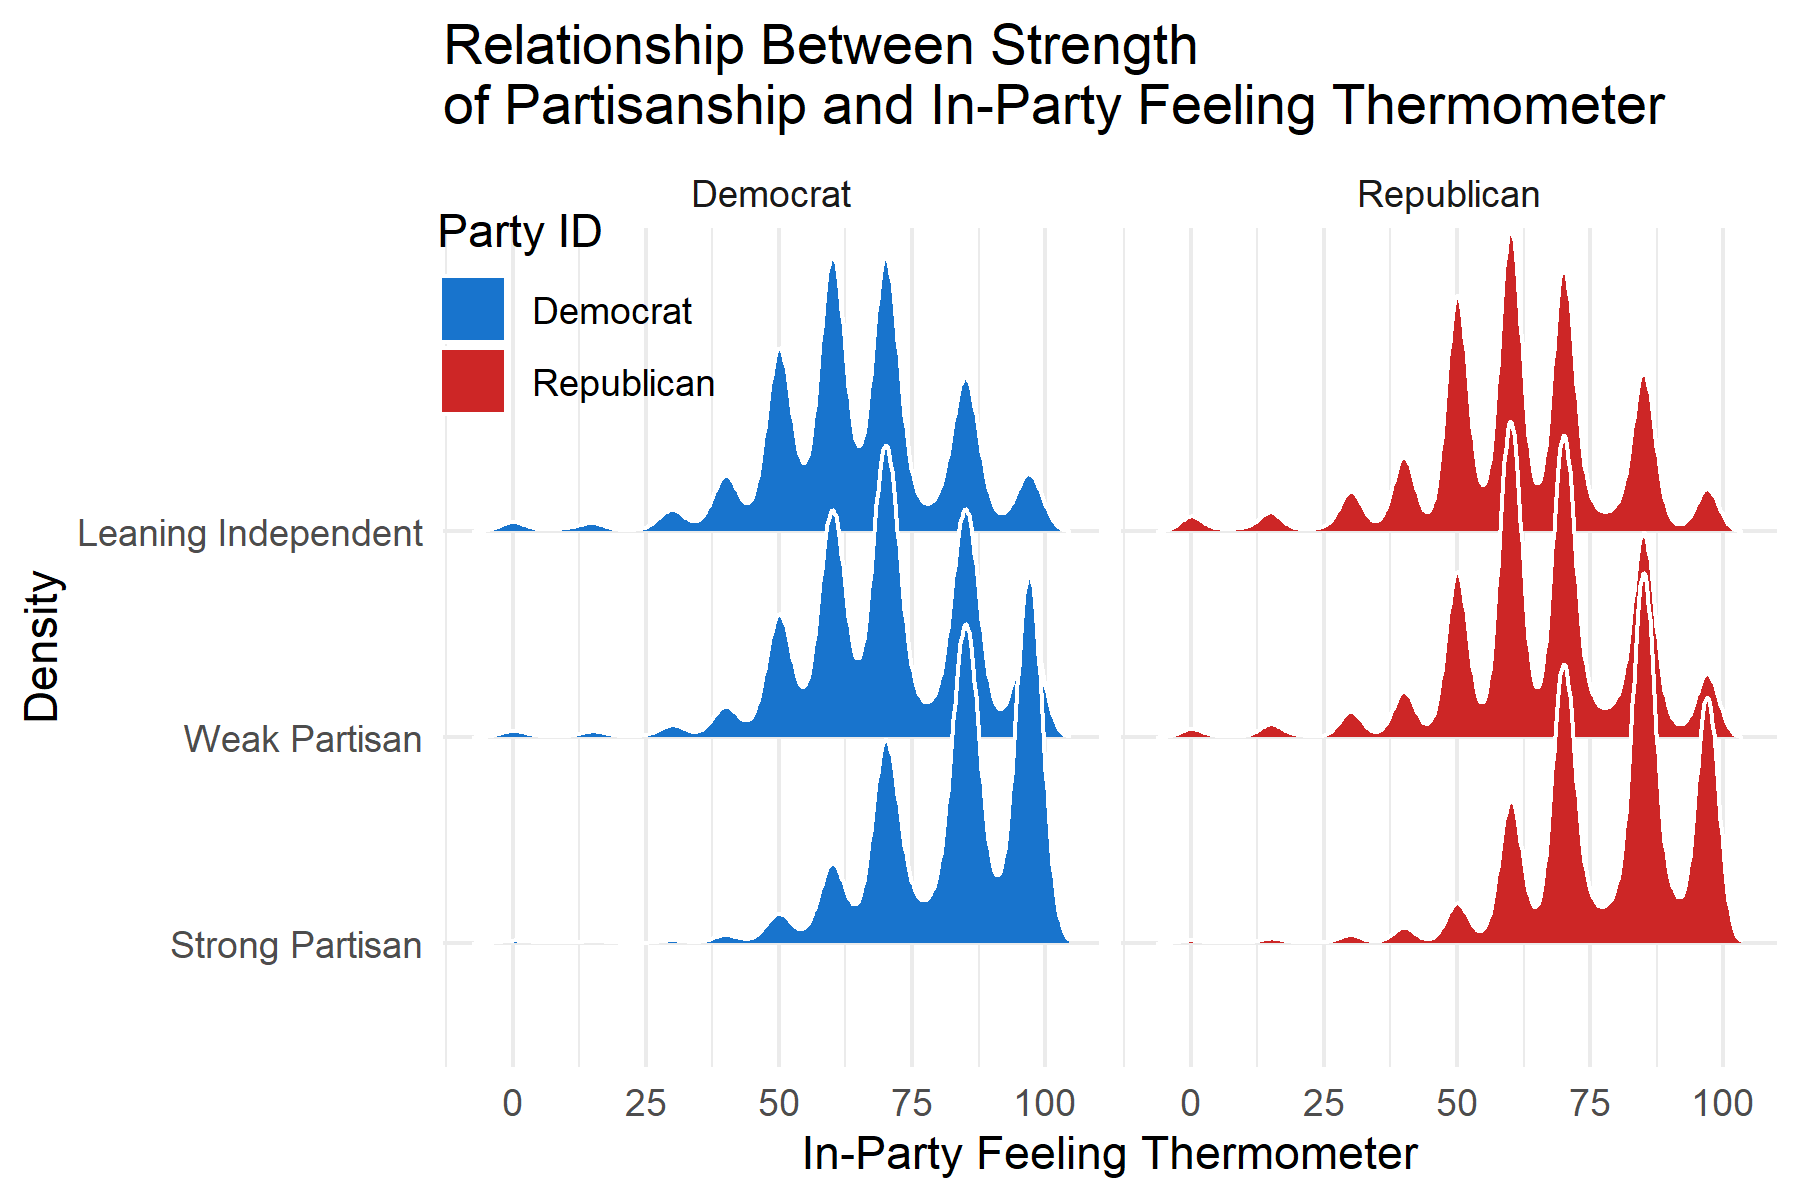
\includegraphics{fig/gg-str-therm.png}
\caption{``Relationship between strength of partisanship and in-party feeling thermometers''}
\end{figure}

\emph{\textbf{Fig SI-2:} There is a positive relationship between partisans' strength of identification and their in-party feeling thermometer ratings.}

\includegraphics{practicum_files/figure-latex/primaries-plots-si-1.pdf} \includegraphics{practicum_files/figure-latex/primaries-plots-si-2.pdf}

\end{document}
